\question[10] Después de leer un libro sobre el antiguo Egipto, Cassie decidió construir con cartón un modelo de una pirámide,
como la que se muestra en la figura \ref{fig:prob_verb_superficie_05}.
\textbf{¿Cuánto cartón necesita Cassie para hacer el modelo, incluyendo la base?}

\begin{minipage}{0.3\linewidth}
    \begin{figure}[H]
        \begin{center}
            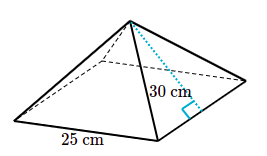
\includegraphics[width=1\textwidth]{../images/prob_verb_superficie_05}
        \end{center}
        \caption{}
        \label{fig:prob_verb_superficie_05}
    \end{figure}
\end{minipage}
\begin{minipage}{0.7\linewidth}
    \begin{solutionbox}{6cm}
        El volumen de un cilindro de radio $r$ y altura $h$ es:
        \begin{equation*}
            V = \pi r^2 h
        \end{equation*}
        De la figura \ref{fig:vol_area_03} se sabe que $r=2$ y $h=5$, entonces
        \begin{equation*}
            \begin{split}
                V & = \pi r^2 h\\
                & = \pi (4)^2 (10)\\
                & = \pi (16) (10)\\
                & = 160\pi
            \end{split}
        \end{equation*}
    \end{solutionbox}
\end{minipage}